\pagebreak
\section{Domain Mapping}
A reference-to-global coordinate mapping $\vec{x}\left(\vec{\xi}\right)$ is given by
\begin{align*}
    x & = \xi + \frac{1}{2}\eta^2,\\
    y & = 1 + \eta - \frac{1}{4}\xi\eta,
\end{align*}

where $\vec{\xi} = \left(\xi, \eta\right)$ and $\vec{x} = \left(x,y\right)$. Consider a unit square domain in reference space, $\vec{\xi}\in [0,1]^2$.

\begin{enumerate}[label = \alph*., start = 1]
    \item Show what this domain looks like in global space by providing a computer-generated plot of the domain edges.
    
    \begin{figure}[h]
        \centering
        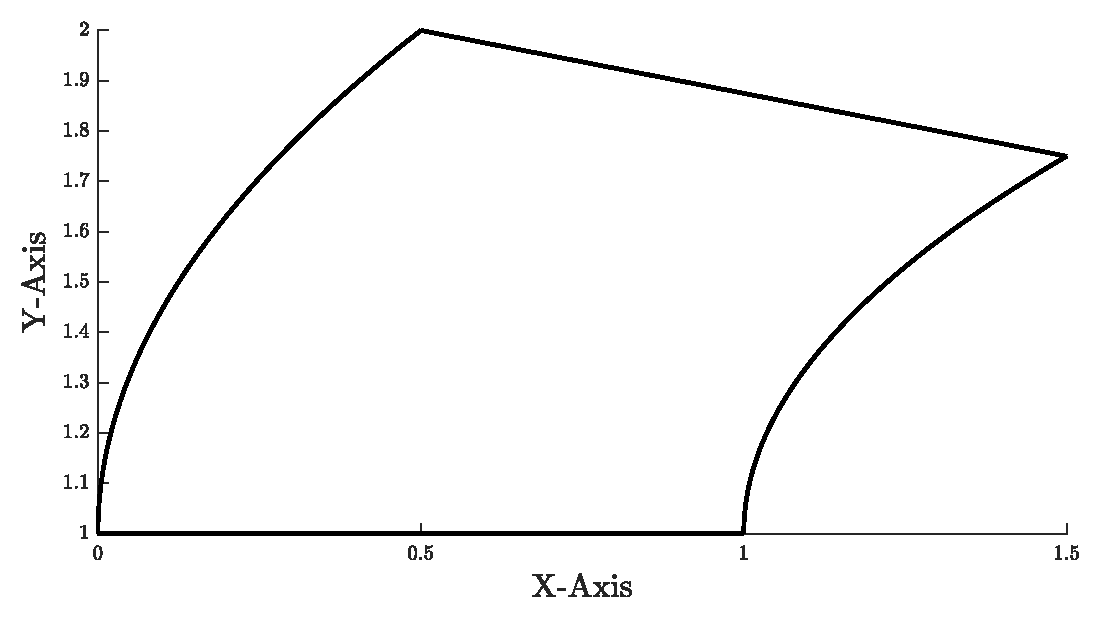
\includegraphics[width = 0.6\linewidth]{q3/domain.eps}
        \caption{Reference space mapped to global space.}
        \label{fig:q3_refspace}
    \end{figure}

    \begin{fminipage}{0.8\linewidth}
        \textbf{Mapping the reference space to the global space results in Figure \ref{fig:q3_refspace} shown above.}
    \end{fminipage}

    \item Determine  an  analytical  expression  for  the  $2\times2$  mapping  Jacobian  matrix, ${\bf J}\equiv \frac{\partial \vec{x}}{\partial \vec{\xi}}$,  and  its determinant, ${\bf J}\equiv \det{\left(\bf J\right)}$.
    
    \vspace{-0.4in}
    \begin{align*}
        \shortintertext{The Jacobian matrix can be written as,}
        J & = \begin{bmatrix} \frac{\partial x}{\partial \xi} & \frac{\partial x}{\partial \eta}\\
        \frac{\partial y}{\partial \xi} & \frac{\partial y}{\partial \eta}\end{bmatrix} = \begin{bmatrix}
            \frac{\partial }{\partial \xi}\left( \xi + \frac{1}{2}\eta^2 \right) & \frac{\partial }{\partial \eta}\left( \xi + \frac{1}{2}\eta^2 \right)\\
            \frac{\partial }{\partial \xi}\left( 1 + \eta - \frac{1}{4}\xi\eta \right) & \frac{\partial }{\partial \eta}\left( 1 + \eta - \frac{1}{4}\xi\eta \right)
        \end{bmatrix}\\
        \shortintertext{Then taking the derivatives give,}
    \end{align*}

    \vspace{-0.5in}
    \begin{equation*}
        \boxed{ \doubleunderline{J} = \begin{bmatrix}
            1 & \eta\\
            -\frac{1}{4}\eta & 1 - \frac{1}{4}\xi
        \end{bmatrix}}
    \end{equation*}
    
    \vspace{-0.4in}
    \begin{align*}
        \shortintertext{Then taking the determinant gives,}
        \det{(J)} & = 1\cdot\left(1 - \frac{1}{4}\xi\right) - \eta\left(-\frac{1}{4}\eta\right)\\
        \shortintertext{This then results in the following determinant result,}
    \end{align*}

    \vspace{-0.5in}
    \begin{equation*}
        \boxed{\det{(J)} = 1 + \frac{1}{4}(\eta^2 - \xi)}
    \end{equation*}

    \pagebreak
    \item Calculate the normal vectors at the four domain edge midpoints (where the midpoint is identified in reference space).
    
    \begin{figure}[h]
        \centering
        

\tikzset{every picture/.style={line width=0.75pt}} %set default line width to 0.75pt        

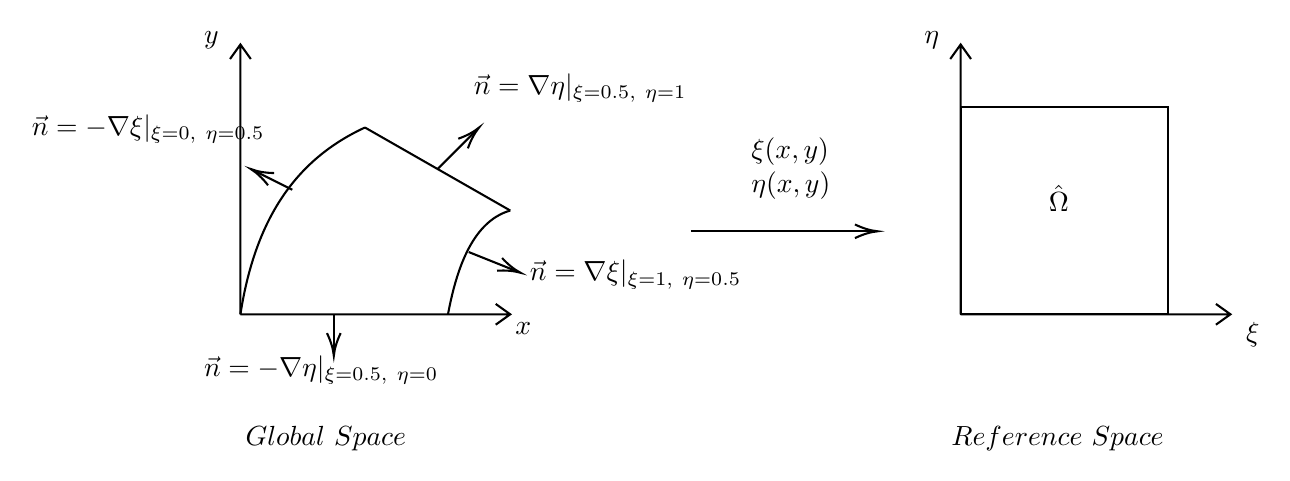
\begin{tikzpicture}[x=0.75pt,y=0.75pt,yscale=-1,xscale=1]
%uncomment if require: \path (0,300); %set diagram left start at 0, and has height of 300

%Shape: Axis 2D [id:dp7380948353026224] 
\draw  (133,180) -- (263,180)(133,50) -- (133,180) -- cycle (256,175) -- (263,180) -- (256,185) (128,57) -- (133,50) -- (138,57)  ;
%Shape: Axis 2D [id:dp8732172960708304] 
\draw  (480,180) -- (610,180)(480,50) -- (480,180) -- cycle (603,175) -- (610,180) -- (603,185) (475,57) -- (480,50) -- (485,57)  ;
%Curve Lines [id:da6439554475328086] 
\draw    (133,180) .. controls (140.5,131.57) and (161.5,104.57) .. (193,90) ;
%Curve Lines [id:da7450361057497594] 
\draw    (233,180) .. controls (236.5,161.57) and (243.5,135.57) .. (263,130) ;
%Straight Lines [id:da701652135230981] 
\draw    (193,90) -- (263,130) ;
%Straight Lines [id:da6822793783891032] 
\draw    (350,140) -- (438,140) ;
\draw [shift={(440,140)}, rotate = 180] [color={rgb, 255:red, 0; green, 0; blue, 0 }  ][line width=0.75]    (10.93,-3.29) .. controls (6.95,-1.4) and (3.31,-0.3) .. (0,0) .. controls (3.31,0.3) and (6.95,1.4) .. (10.93,3.29)   ;
%Shape: Square [id:dp347937538101061] 
\draw   (480,80) -- (580,80) -- (580,180) -- (480,180) -- cycle ;
%Straight Lines [id:da44592555123633604] 
\draw    (228,110) -- (246.59,91.41) ;
\draw [shift={(248,90)}, rotate = 495] [color={rgb, 255:red, 0; green, 0; blue, 0 }  ][line width=0.75]    (10.93,-3.29) .. controls (6.95,-1.4) and (3.31,-0.3) .. (0,0) .. controls (3.31,0.3) and (6.95,1.4) .. (10.93,3.29)   ;
%Straight Lines [id:da7188497207060873] 
\draw    (243,150) -- (266.14,159.26) ;
\draw [shift={(268,160)}, rotate = 201.8] [color={rgb, 255:red, 0; green, 0; blue, 0 }  ][line width=0.75]    (10.93,-3.29) .. controls (6.95,-1.4) and (3.31,-0.3) .. (0,0) .. controls (3.31,0.3) and (6.95,1.4) .. (10.93,3.29)   ;
%Straight Lines [id:da20467386352369865] 
\draw    (178,180) -- (178,198) ;
\draw [shift={(178,200)}, rotate = 270] [color={rgb, 255:red, 0; green, 0; blue, 0 }  ][line width=0.75]    (10.93,-3.29) .. controls (6.95,-1.4) and (3.31,-0.3) .. (0,0) .. controls (3.31,0.3) and (6.95,1.4) .. (10.93,3.29)   ;
%Straight Lines [id:da37405110877950887] 
\draw    (158,120) -- (139.79,110.89) ;
\draw [shift={(138,110)}, rotate = 386.57] [color={rgb, 255:red, 0; green, 0; blue, 0 }  ][line width=0.75]    (10.93,-3.29) .. controls (6.95,-1.4) and (3.31,-0.3) .. (0,0) .. controls (3.31,0.3) and (6.95,1.4) .. (10.93,3.29)   ;

% Text Node
\draw (371,92.4) node [anchor=north west][inner sep=0.75pt]    {$ \begin{array}{l}
\xi ( x,y)\\
\eta ( x,y)
\end{array}$};
% Text Node
\draw (264,182.4) node [anchor=north west][inner sep=0.75pt]    {$x$};
% Text Node
\draw (114,42.4) node [anchor=north west][inner sep=0.75pt]    {$y$};
% Text Node
\draw (461,42.4) node [anchor=north west][inner sep=0.75pt]    {$\eta $};
% Text Node
\draw (616,182.4) node [anchor=north west][inner sep=0.75pt]    {$\xi $};
% Text Node
\draw (521,116.4) node [anchor=north west][inner sep=0.75pt]    {$\hat{\Omega }$};
% Text Node
\draw (134,232.4) node [anchor=north west][inner sep=0.75pt]    {$Global\ Space$};
% Text Node
\draw (474,232.4) node [anchor=north west][inner sep=0.75pt]    {$Reference\ Space$};
% Text Node
\draw (31,82.4) node [anchor=north west][inner sep=0.75pt]    {$\vec{n} =-\nabla \xi |_{\xi =0,\ \eta =0.5}$};
% Text Node
\draw (114,198.4) node [anchor=north west][inner sep=0.75pt]    {$\vec{n} =-\nabla \eta |_{\xi =0.5,\ \eta =0}$};
% Text Node
\draw (244,62.4) node [anchor=north west][inner sep=0.75pt]    {$\vec{n} =\nabla \eta |_{\xi =0.5,\ \eta =1}$};
% Text Node
\draw (271,152.4) node [anchor=north west][inner sep=0.75pt]    {$\vec{n} =\nabla \xi |_{\xi =1,\ \eta =0.5}$};


\end{tikzpicture}

        \caption{Global to Reference space transformation.}
        \label{fig:spaces}
    \end{figure}

    In order to compute the normal vectors in the global space with reference to the mid-points in the reference space, I will solve for the expressions for $\xi$ and $\eta$. Conducting this in Matlab and simplifying gives that $\xi$ and $\eta$ are,

    \begin{gather*}
        \xi = \input{q3/xi_exp}\\
        \eta = \input{q3/eta_exp}
    \end{gather*}

    With $\xi$ and $\eta$ having been solved for, the normal vectors can be solved for by taking the gradient at the mid-points of the references as shown in Figure \ref{fig:spaces}. With the expressions for $\xi$ and $\eta$ in terms of $x$ and $y$ so taking the gradient at each respective reference midpoint through Matlab gives that the normal vectors are,

    \begin{fminipage}{0.3\linewidth}
        \begin{align*}
            \input{q3/n_output}
        \end{align*}    
    \end{fminipage}
    
    \pagebreak
    \item Calculate the area of the domain in global space by an analytical integration over the reference unit square.
    
    Integrating over the global domain by using the transformation from the reference domain. The integral of some function $f(\vec{x})$ transforms as,
    \begin{equation*}
        \int_{\Omega}f(\vec{x})\ dxdy = \int_{\hat{\Omega}}f\left(\vec{x}\left(\vec{\xi}\right)\right)\det{(J)}\ d\xi d\eta
    \end{equation*}

    Since the area in global space can be represented in the reference domain, then this integration can be simplified significantly. In other words this can be an integration above the top of the reference unit-square where $\xi$ can vary and $\eta = 1$. This gives that the function $f\left(\vec{x}\left(\vec{\xi}\right)\right)=1$
     
    Re-writing and substituting in the determinant of the Jacobian gives,

    \vspace{-0.35in}
    \begin{align*}
        A_{\Omega} & = \int_{\partial \hat{\Omega}} \underbrace{1 + \frac{1}{4}(\eta^2 - \xi)}_{\det{(J)}}\ d\xi d\eta\\
        \shortintertext{Where the domains are $\xi \in [0,1]$ and $\eta \in [0, 1]$, simplifying gives,}
        A_{\Omega} & = \int_{\eta = 0}^{\eta = 1}\int_{\xi = 0}^{\xi = 1} 1 + \frac{1}{4}(\eta^2 - \xi)\ d\xi d\eta\\
        \shortintertext{Conducting the integral gives,}
        A_{\Omega} & = \int_{\eta = 0}^{\eta = 1} \left(\xi + \frac{1}{4}\eta^2\xi - \frac{1}{8}\xi^2\right)|_{\xi = 0}^{\xi = 1}\ d\eta\\
            & = \int_{\eta = 0}^{\eta = 1} 1 + \frac{1}{4}\eta^2 - \frac{1}{8}\ d\eta\\
            & = \int_{\eta = 0}^{\eta = 1} \frac{7}{8} + \frac{1}{4}\eta^2\ d\eta\\
            & = \frac{7}{8}\eta + \frac{1}{12}\eta^3|_{\eta = 0}^{\eta = 1}\\
            & = \frac{7}{8} + \frac{1}{12}\\
        \shortintertext{This gives that the area in the global space is,}
    \end{align*}

    \vspace{-0.35in}
    \begin{equation*}
        \boxed{A_{\Omega} = \frac{23}{24}}
    \end{equation*}
\end{enumerate}